\documentclass{beamer}
\usepackage[utf8]{inputenc}
\usepackage{hyperref}

\usepackage{tikz}

\usepackage{latexsym,xcolor,multicol,booktabs,calligra}
\usepackage{amsmath,amssymb,BOONDOX-cal,bm}	
\usepackage{graphicx,pstricks,stackengine} 
\usepackage{libertinus}
\usepackage{amssymb}
\usepackage{pgfplots}
\usepackage{tikz}
\usepackage{xcolor}
\usetikzlibrary{positioning}

\usepackage{etoolbox}
\makeatletter
\newcommand{\noframenumbering}{%
  \beamer@noframenumberingtrue%
}
\makeatother

\usepackage[T1]{fontenc}

\title{Macroeconometrics\\
4 - VAR}
\author{Camille Souffron\\
Ecole Normale Supérieure \& Paris School of Economics\\
\textcolor{blue}{\href{mailto:camille.souffron@ens.psl.eu}{camille.souffron@ens.psl.eu}}}
\institute{\normalsize M2 EPOG JM}
\date{Fall 2026}

\usetheme{Singapore}

\def\cmd#1{\texttt{\color{red}\footnotesize $\backslash$#1}}
\def\env#1{\texttt{\color{RoyalBlue}\footnotesize #1}}

\newtheorem{thm}{Theorem}[theorem]
\setbeamertemplate{footline}[frame number]

\begin{document}

\begin{frame} % <-- no [plain] here!
    \titlepage % This keeps the theme style
    \begin{center}
        
\includegraphics[width=0.5\textwidth]{logos.png}
    \end{center}
\end{frame}



\addtocounter{framenumber}{-1}


% =====================================================
% WHAT WE HAVE LEARNED SO FAR — ARMA (PART I)
% =====================================================
\begin{frame}{What We Have Learned So Far (ARMA - Part I)}
\scriptsize
\begin{enumerate}
\item \textbf{From Stationarity to Dynamic Modelling}
  \begin{itemize}
  \scriptsize
    \item Once the series is stationary (no trend, constant variance, $\gamma(h)$ depends only on $h$), we can model its dynamics statistically.
    \item \textbf{Wold Theorem:} any weakly stationary process admits a linear MA($\infty$) representation $          X_t = \mu + \sum_{j=0}^{\infty} \psi_j \varepsilon_{t-j}$
    \item Finite, parsimonious approximations $\Rightarrow$ AR($p$), MA($q$), ARMA($p,q$) models.
    \item For integrated processes (non-stationary with a unit root), we difference $d$ times: $(1-L)^d X_t = \text{stationary process} \Rightarrow X_t \sim \text{ARIMA}(p,d,q)$ where $d$ is the number of first differences required to reach stationarity.
  \end{itemize}

    \pause
\item \textbf{Lag Operator and Lag Polynomials}
  \begin{itemize}
  \scriptsize
    \item Lag operator: $L X_t = X_{t-1}$, $L^k X_t = X_{t-k}$.
    \item AR($p$): $\phi(L)X_t = \mu + \varepsilon_t$, with $\phi(L) = 1-\phi_1L-\cdots-\phi_pL^p$.
    \item MA($q$): $X_t = \mu + \theta(L)\varepsilon_t$, with $\theta(L) = 1-\theta_1L-\cdots-\theta_qL^q$.
    \item \textbf{Stationarity (AR part):} all roots of $\phi(z)=0$ satisfy $|z_i|>1$ (equivalently $|\lambda_i|<1$ for $\lambda_i = 1/z_i$) $\Rightarrow$ past shocks decay geometrically.
    \item \textbf{Invertibility (MA part):} all roots of $\theta(z)=0$ satisfy $|z_i|>1$ $\Rightarrow$ the innovation sequence $(\varepsilon_t)$ is uniquely identified. \textbf{NB:} MA processes are \emph{always stationary}.
  \end{itemize}
    \pause
\item \textbf{Interpretation and Forecasting Motivation}
  \begin{itemize}
  \scriptsize
    \item AR part $\Rightarrow$ feedback and persistence; MA part $\Rightarrow$ short-term noise smoothing.
    \item Stationary + invertible $\Rightarrow$ mean reversion, and exponential damping of shocks.
    \item ARMA $\Rightarrow$ finite-order approximation of the \textbf{Best Linear Forecast (BLF)} minimizing the mean-squared forecast error $ \min_{\{\alpha_j\}} E[(X_{t+h} - \sum_j \alpha_j X_{t-j})^2]$  with the optimality (orthogonality) condition $\text{Cov}(\widehat{\varepsilon}_t(h),\, X_{t-j}) = 0 \quad \forall j \ge 0.$
  \end{itemize}
\end{enumerate}
\end{frame}


% =====================================================
% WHAT WE HAVE LEARNED SO FAR — ARMA (PART II)
% =====================================================

\begin{frame}{What We Have Learned So Far (ARMA - Part II)}
\scriptsize
\begin{enumerate}
\setcounter{enumi}{3}
\item \textbf{Identification of Model Orders $(p,q)$}
  \begin{itemize}
  \scriptsize
    \item Use sample ACF and PACF (\textit{Partial} ACF) to identify lag structures:
      \begin{itemize}
        \scriptsize
        \item AR($p$): ACF decays exponentially, PACF cuts off after lag $p$.
        \item MA($q$): ACF cuts off after lag $q$, PACF decays exponentially.
        \item ARMA($p,q$): both ACF and PACF decay gradually.
      \end{itemize}
    \item These patterns provide first guesses for $(p,q)$ before estimation.
  \end{itemize}
    \pause
\item \textbf{Estimation and Model Selection}
  \begin{itemize}
  \scriptsize
    \item AR($p$): estimated by \textbf{OLS} (predetermined regressors, consistent). 
    \item MA/ARMA: estimated via \textbf{MLE} (or \textbf{NLS}) since latent $\varepsilon_{t-i}$.
    \item Select $(p,q)$ by \textbf{minimizing information criteria} (AIC/BIC/HQC) for an optimal bias-variance (misspecification-overfitting) trade-off.
  \end{itemize}
    \pause
\item \textbf{Model Validation (Residual Diagnostics)}
  \begin{itemize}
  \scriptsize
    \item Once the preferred model (lowest IC) is chosen, check that residuals are white noise:
      \begin{itemize}
        \scriptsize
        \item \textbf{Ljung-Box} ($H_0$: no autocorrelation up to lag $m$) - ensures model used all useful linear info.
        \item         Plot residual ACF: $\approx 0$ $\Rightarrow$ white noise, hence model adequate (\textbf{we used all the useful information from the past, thus current error = white noise)}.\textbf{ If auto-correlation: need more lags!}
        \item \textbf{Jarque-Bera} ($H_0$: normality) - needed only for exact finite-sample inference. \textbf{Q-Q plot:} graphical check for normality (45° line $\Rightarrow$ Gaussian WN; S-shape $\Rightarrow$ heavy tails or skewness).

      \end{itemize}
  \end{itemize}
\end{enumerate}
\end{frame}


% =====================================================
% WHAT WE HAVE LEARNED SO FAR — ARMA (PART III)
% =====================================================

\begin{frame}{What We Have Learned So Far (ARMA - Part III)}
\scriptsize
\begin{enumerate}
\setcounter{enumi}{6}

\item \textbf{Forecasting}
  \begin{itemize}
  \scriptsize
    \item Forecast recursively (future $\varepsilon_{t+h}=0$), with 
          $Var(e_{T+h|T}) = \sigma^2 \sum_{i=0}^{h-1}\psi_i^2$.
    \item Evaluate predictive accuracy: RMSE, MAE, MSE on \textbf{rolling or expanding windows.}
    \item Use \textbf{bootstrap} for forecast confidence intervals.
    \item \textbf{\textit{Asymptotic forecast limit (stationary ARMA):}} as $h\!\to\!\infty$, 
          $\widehat{X}_{T}(h)\!\to\!\mu$ (unconditional mean. $0$ if $\mu=0$) and 
          $Var(e_{T+h|T}) \!\to\! Var(X_t) = \sigma^2 \sum_{i=0}^{\infty}\psi_i^{\,2}$. Since \textbf{LINEAR} model (either converges if stationary, or explodes).
\end{itemize}
    \pause
    \item \textbf{Regime Changes \& Overfitting}
  \begin{itemize}
  \scriptsize
    \item \textbf{\textit{Window-length vs regime shifts:}} longer samples improve efficiency\textbf{ \textit{only if}} the DGP is stable. 
          With structural change, use \textbf{rolling} or \textbf{recent} windows.
    \item \textbf{\textit{Break tests (mean/variance):}} 
    \begin{itemize}
      \scriptsize
        \item Known-date mean break (Chow); multiple unknown breaks (supF Bai-Perron / \texttt{strucchange}).\\
        \item Check volatility clustering via ARCH tests (e.g. Engle LM or LB on $\hat{\varepsilon}_t^2$), variance breaks (\texttt{changepoint} PELT). ARCH/GARCH = heteroskedastic variance model.
    \end{itemize}
\textbf{\item \textit{Overfitting risk:}} more terms lower in-sample error but raises out-of-sample error. 
  \end{itemize}
\end{enumerate}
\end{frame}

%======================================================
\begin{frame}{NB: comparing unit root tests}
%======================================================
\tiny
\textbf{Always specify:} the series have a \textbf{deterministic trend} (trend-stationary) 
or only\textbf{ a constant mean (mean-stationary)}? Must be run with the appropriate deterministic component. Disagreement $\Rightarrow$ near-unit-root or structural break.
Always report deterministic term (\textit{none / constant / trend}) and chosen lag length.

\begin{tabular}{p{1.7cm}p{2.4cm}p{2.6cm}p{3.3cm}}
\toprule
\textbf{Test} & \textbf{Null Hypothesis ($H_0$)} & \textbf{Correction / Feature} & \textbf{Use or Limitation} \\
\midrule
\textbf{ADF} (Augmented Dickey-Fuller)&
Unit root (non-stationary) &
Adds lags of $\Delta y_t$ to absorb autocorrelation. &
Simple benchmark; sensitive to lag choice; assumes homoskedasticity. \\[0.1cm]

\textbf{PP} (Phillips-Perron)&
Unit root &
Nonparametric correction (Newey-West) for serial correlation and heteroskedasticity.&
Robust to residual dynamics, but does \emph{not} detect breaks. \\[0.1cm]

\textbf{KPSS} (Kwiatkowski-Phillips-Schmidt-Shin)&
Stationarity (no unit root) &
Tests whether long-run variance of a random walk component is zero. &
Complementary to ADF/PP; can over-reject under breaks. \\[0.1cm]

\textbf{ZA} (Zivot-Andrews)&
Unit root with a structural break&
Allows one break in trend or intercept within the sample. &
Useful if structural change suspected; lower power in small $n$. \\[0.1cm]

\textbf{ERS / DF-GLS} (Elliott-Rothenberg-Stock)&
Unit root &
GLS-detrends series before ADF regression. &
Higher power in finite samples; sensitive to trend specification. \\
\bottomrule
\end{tabular}


\end{frame}

\section{Introduction}


\begin{frame}{Motivating questions for VARs}

\begin{enumerate}
    \item How to consider a multivariate framework (i.e. \textit{\textbf{vector} auto-regression - VAR})? 
    \begin{enumerate}
        \item  A single series cannot capture how macroeconomic variables interact.
    \end{enumerate}
    \begin{enumerate}

        \item Macroeconomic systems are \textit{jointly} determined
        \item Output, inflation, interest rates, credit, investment, unemployment, etc. are \emph{simultaneously evolving}.  
    \end{enumerate}
    \pause
    \item Can we not only forecast the future, but also simulate the impact of a policy / a shock in a causal, \textbf{"structural"} way? (i.e. \textit{impulse response function (IRF) in structural VAR}). 
    \begin{enumerate}
        \item The \textit{\textbf{identification}} problem.
        \item No single variable is exogenous in macro data; \textbf{feedback} is pervasive.
    \item A shock to one variable propagates through the entire system.
    \end{enumerate}
        \pause
    \item Can we quantify the \textbf{contribution of each variable}:
    \begin{enumerate}
        \item  to the overall variance (i.e. \textit{variance decomposition}), and 
        \item to the prediction accuracy (i.e.\textit{ Granger causality})?
    \end{enumerate}
\end{enumerate}
\end{frame}


\begin{frame}{\textit{Macroeconomics and Reality }}
\footnotesize
"Macroeconomics and Reality" (Christopher Sims, 1980, Econometrica): \textit{foundations} of modern macroeconometrics (gave him a Nobel).

\smallskip
\textbf{In 1980, macroeconometrics was dominated by:}
\medskip

\textbf{Large-Scale Structural Econometric Models (SEMs)}
\begin{itemize}
    \item FRB-MIT-Penn, Brookings, Wharton models.
    \item "Disequilibrium Theory" or\textit{ non-Walrasian} equilibrium theory (neo-classical-keynesian synthesis: Patinkin, Malinvaud \& Benassy, Clower \& Leijonhufvud, Tobin, Modigliani...). Cf. \textit{Transforming Modern Macroeconomics: Exploring Disequilibrium Microfoundations}, 1956-2003 (2012). Cf. Barro-Grossman model (1971).
    \item Hundreds of equations, each with strong "theoretical" restrictions (\textit{ad hoc}).
    \item Identification through \emph{a priori} exclusion restrictions.
    \item Claimed to deliver policy simulations and causal statements.
\end{itemize}

\medskip
\textbf{Sims’ diagnosis:}
\begin{itemize}
    \item Poor predictive performance in the 1970s (oil shocks, stagflation).
    \item Identifying assumptions often \emph{arbitrary} and \emph{not credible}.
    \item Causality/exogeneity was imposed by the modeler rather than the data.
    \item SEMs implicitly assumed that the econometrician "knows the true structure."
\end{itemize}
\end{frame}

\begin{frame}{\textit{Macroeconomics and Reality }}
\footnotesize
\textbf{Lucas (1976): The Lucas Critique}
\begin{itemize}
    \item Structural parameters depend on policy regimes.
    \item Traditional SEMs are not policy-invariant $\Rightarrow$ unreliable for policy!
\end{itemize}

\textbf{Sargent \& Wallace (1975) and \textit{fresh water} macroeconomics}
\begin{itemize}
    \item Rational expectations (and policy ineffectiveness proposal - PII).
    \item "Microfounded" structural equations.
    \item Identification grounded in theory rather than data.
\end{itemize}
\textbf{Results: RBC (Real Business Cycle)} models ("microfounded"\footnote{\scriptsize Really "microfounded"? Kirman (1992, JEP): "Whom or What Does the Representative Individual Represent?"} optimising GE models calibrated to reproduce empirical co-movements), Kydland \& Prescott (1982); Long \& Plosser (1983).
\medskip

\begin{itemize}
    \item \textbf{Sims’ view: }Lucas and Sargent are correct to criticize old structural models.
    \item But their alternative introduces \emph{even stronger} and often
          \emph{untestable} assumptions (Rational expectations, Euler equation, market clearing etc.)
    \item Empirical macro needs a third way: 
    \begin{itemize}
    \footnotesize
        \item \textbf{agnostic statistical structure (crossed autoregressive, i.e. VAR), 
        \item and identification without unrealistic theoretical constraints.}
    \end{itemize}
\end{itemize}

\end{frame}



\begin{frame}{\textit{Macroeconomics and Reality }}
%======================================================
\footnotesize
\textbf{1. Sims’ Approach (empirical workhorse of macroeconometric)}
\begin{itemize}
    \item Treats \emph{all} macro variables as jointly endogenous (no “exogeneity by assumption”).
    \item Starts from the reduced form: \textbf{unrestricted VAR}.
    \item Identifies shocks using \textbf{minimal}, transparent assumptions: recursive (Cholesky) timing rules or information-set arguments.
    \item Uses the VAR’s VMA representation to compute \textbf{impulse response functions} (IRFs) and
          \textbf{forecast error variance decompositions} (FEVDs) for dynamic analysis.
          \item Responds to the Lucas Critique \emph{without} requiring full microfoundations.
\end{itemize}

\bigskip

\textbf{2. Empirical Results}
\begin{itemize}
    \item Money is not exogenous: monetary aggregates respond endogenously to the economy vs monetarist SEMs.
    \item VAR-based IRFs differ sharply from predictions of SEMs (timing, magnitude) e.g. some variables (prices) adjust faster.
    \item Output, prices, unemployment, and money show richer dynamics (e.g. money reacts to unemployment and inflation, not the reverse only)
    \item Shows simple VARs can outperform large SEMs in short-run forecasting.
\end{itemize}

\end{frame}



\section{VAR}


%======================================================
\begin{frame}{Vector Autoregression}
%======================================================
For now, we do not consider identification / causality / structural VAR. We consider only \textbf{\textit{reduced-form}} VAR.
\bigskip

\textbf{Vector Autoregressions (VARs):} a minimal, flexible multivariate framework
\begin{itemize}
    \item Treat all variables as jointly endogenous (cross-equations (terms in all equations)).
    \item Model their dynamics using only \textbf{lagged values} of all variables (\textit{autoregressive})
\end{itemize}
\end{frame}


%======================================================
\begin{frame}{The VAR$(p)$ Model: Definition and Notation}
%======================================================
\small

\textbf{The Multivariate Extension of AR Models}

\medskip
Let $y_t$ be a $k \times 1$ vector of jointly endogenous variables.  

A \textbf{Vector Autoregression of order $p$} is:

\[
\underbrace{y_t}_{k\times 1}
= 
\underbrace{c}_{k\times 1}
+
\underbrace{A_1 y_{t-1} + \cdots + A_p y_{t-p}}_{k\times 1}
+
\underbrace{B x_t}_{k\times 1}
+
\underbrace{u_t}_{k\times 1}
\]

\begin{itemize}
    \item $c$ : intercept vector (deterministic).  
    \item $A_i$ : $k \times k$ autoregressive coefficient matrices.  
    \item $x_t$ : $r \times 1$ optional exogenous controls (\textbf{VARX}), $B :(k\times r$)
    \item $u_t$ : reduced-form innovations, with $u_t \sim (0, \Sigma_u)$.
\end{itemize}

\bigskip

\begin{itemize}
    \item Each variable depends on \emph{its own lags} and on the \emph{lags of all other variables}.
    \item All variables are treated symmetrically\textbf{ (no a priori “endogenous/exogenous” distinction).}
\end{itemize}
\end{frame}


%======================================================
\begin{frame}{Example: 3-Variable VARX(1)\\(GDP growth, Inflation, Interest rate)}
%======================================================
\small

Let the endogenous vector be:
\[
y_t =
\begin{pmatrix}
g_t \\ \pi_t \\ i_t
\end{pmatrix},
\quad
\begin{aligned}
g_t &: \text{GDP growth},\\
\pi_t &: \text{Inflation},\\
i_t &: \text{Interest rate}.
\end{aligned}
\]
Let the exogenous controls be:
\[
x_t =
\begin{pmatrix}
\Delta \text{Oil}_t \\ \text{Policy}_t
\end{pmatrix},
\qquad (r=2).
\]

\medskip

A VARX(1) is:
\[
y_t = c + A_1 y_{t-1} + B x_t + u_t,
\quad
c \in \mathbb{R}^{3\times 1},\ 
A_1 \in \mathbb{R}^{3\times 3},\ 
B \in \mathbb{R}^{3\times 2}.
\]

\[
A_1 =
\begin{pmatrix}
a_{11} & a_{12} & a_{13} \\
a_{21} & a_{22} & a_{23} \\
a_{31} & a_{32} & a_{33}
\end{pmatrix},
\qquad
B =
\begin{pmatrix}
b_{11} & b_{12} \\
b_{21} & b_{22} \\
b_{31} & b_{32}
\end{pmatrix}.
\]


\end{frame}


%======================================================
\begin{frame}{Example: 3-Variable VARX(1)\\(GDP growth, Inflation, Interest rate)}
%======================================================
Let's write the developed system (\textbf{component equations}):
\pause

\[
\begin{aligned}
g_t &= c_1 + a_{11} g_{t-1} + a_{12} \pi_{t-1} + a_{13} i_{t-1}
      + b_{11}\Delta \text{Oil}_t + b_{12}\text{Policy}_t + u_{1t},\\[4pt]
\pi_t &= c_2 + a_{21} g_{t-1} + a_{22} \pi_{t-1} + a_{23} i_{t-1}
      + b_{21}\Delta \text{Oil}_t + b_{22}\text{Policy}_t + u_{2t},\\[4pt]
i_t &= c_3 + a_{31} g_{t-1} + a_{32} \pi_{t-1} + a_{33} i_{t-1}
      + b_{31}\Delta \text{Oil}_t + b_{32}\text{Policy}_t + u_{3t}.
\end{aligned}
\]

\end{frame}



%======================================================
\begin{frame}{Companion Form and Stability of a VAR$(p)$}
%======================================================
\small

\textbf{Why Companion Form?}  
It converts a VAR$(p)$ into a first-order VAR, making  
\emph{stability, forecasting, and IRFs} analytically tractable.

\medskip

Define the $kp \times 1$ stacked state vector $Y_t =
\begin{pmatrix}
y_t \\ y_{t-1} \\ \vdots \\ y_{t-p+1}
\end{pmatrix}$

Then the VAR$(p)$ can be rewritten as: $Y_t = 
F Y_{t-1} +
\begin{pmatrix}
c \\ 0 \\ \vdots \\ 0
\end{pmatrix}
+
\begin{pmatrix}
u_t \\ 0 \\ \vdots \\ 0
\end{pmatrix}$ 
where $F$ is the \textbf{companion matrix}:

\[
F =
\begin{pmatrix}
A_1 & A_2 & \cdots & A_{p-1} & A_p \\
I_k & 0   & \cdots & 0       & 0 \\
0   & I_k & \cdots & 0       & 0 \\
\vdots &   & \ddots &        & \vdots \\
0   & 0   & \cdots & I_k     & 0
\end{pmatrix}
\]

\end{frame}



%======================================================
\begin{frame}{Stability Condition and VMA Representation}
%======================================================
\small

A VAR$(p)$ is \textbf{stable} \textbf{(i.e.\ weakly stationary)} iff:
\[
\text{all eigenvalues of } F \text{ lie strictly inside the unit circle.}
\]

\medskip

Equivalent condition via the lag polynomial:
\[
A(z) = I_k - A_1 z - A_2 z^2 - \cdots - A_p z^p.
\]
The VAR is stable iff $\det A(z) \neq 0 \quad \text{for all } |z| \leq 1$.
\medskip
\pause
\textbf{Consequences of Stability}

If the VAR is stable, it admits a \textbf{VMA($\infty$) representation} (multivariate generalisation of the \textbf{Wold Decomposition Theorem}).
\[
y_t = \mu + \sum_{h=0}^{\infty} \Phi_h u_{t-h},
\qquad
\Phi_0 = I_k,\;\;
\Phi_h = A_1 \Phi_{h-1} + \cdots + A_p \Phi_{h-p}.
\]

\begin{itemize}
    \item  Thus, a stable VAR($p$) must be a parametric structure being solution to this representation.
    \item $\{\Phi_h\}$ describe dynamic propagation of shocks.
    \item Basis for impulse-response functions (IRFs) and variance decompositions (FEVD).
\end{itemize}
\end{frame}

%======================================================
\begin{frame}{Why Eigenvalues $<1$ $\Rightarrow$ Stability}
%======================================================
\small

\textbf{1) Switch off the shocks (homogeneous system):}
\[
Y_t = F Y_{t-1} \quad \Rightarrow \quad Y_t = F^t Y_0.
\]
Future states depend on repeated applications of $F$.

\medskip
\textbf{2) Stability:}
\[
\text{Stable} \iff \lim_{t\to\infty} F^t Y_0 = 0
\quad \forall\, Y_0.
\]
$\Rightarrow$ Effects of initial conditions vanish over time.

\medskip
\textbf{3) Key property of powers of a matrix:}
If $F = P \Lambda P^{-1}$ (diagonalizable), then
\[
F^t = P \Lambda^t P^{-1},
\qquad
\Lambda^t = \mathrm{diag}(\lambda_1^t,\lambda_2^t,\dots,\lambda_{kp}^t).
\]

\medskip
\textbf{4) Behavior of eigenvalues as $t\to\infty$:}
\[
|\lambda_i|<1 \Rightarrow \lambda_i^t\!\to 0
\quad
|\lambda_i|=1 \Rightarrow \text{persistent}
\quad
|\lambda_i|>1 \Rightarrow \text{explosive}.
\]

\medskip
\textbf{Therefore:}
\[
F^t \to 0
\quad \Leftrightarrow \quad
|\lambda_i|<1 \;\; \forall i.
\]

\textbf{→ The VAR is stable} iff \textbf{all eigenvalues of $F$ lie strictly inside the unit circle.}

\end{frame}


%======================================================
\begin{frame}{How many variables to choose? }
%======================================================
\scriptsize
We want to select a set of endogenous variables that captures key dynamics
without losing degrees of freedom or interpretability. \textbf{A theory-driven choice!}

\begin{tabular}{p{3.3cm}p{7.8cm}}
%======================================================
\scriptsize
\toprule
\textbf{Issue} & \textbf{Implication / Rule of Thumb} \\
\midrule
\textbf{Parameter explosion} &
Each variable adds $k \times p$ new coefficients (for $k$ variables and $p$ lags). \newline
$\Rightarrow$ Total parameters $\approx k^2 p + k$. \newline
Too many variables $\Rightarrow$ few degrees of freedom, large standard errors, poor estimation. \\[0.2cm]

\textbf{Rule of thumb} &
Require at least $T / (k^2 p) > 5$-10 (enough observations per parameter). \newline
Quarterly data ($T\!\approx\!120$) $\Rightarrow$ usually $k \le 4$-5. \\[0.2cm]

\textbf{Interpretability} &
Beyond a few variables, IRFs and FEVDs become opaque. \newline
Shocks mix multiple channels (demand, financial, price), making economic meaning unclear. \\[0.2cm]

\textbf{Identification issues} &
Adding variables complicates ordering and exogeneity assumptions (e.g.\ in Cholesky decomposition). \\[0.2cm]

\textbf{Best practice} &
Start from a clear \textbf{theoretical core} (e.g.\ demand and distribution variables).
Add variables stepwise for robustness (e.g.\ financial indicators).
Check if key impulse responses remain stable.
 Justify omissions explicitly: parsimony $\neq$ arbitrariness.
\\[0.1cm]
\bottomrule
\end{tabular}

\end{frame}


\section{Estimation and Selection}

%======================================================
\begin{frame}{Estimation of a VAR($p$)}
%======================================================

We observe $\{y_t\}_{t=1}^T$ with $y_t\in\mathbb{R}^k$.  To form the regressors $(y_{t-1},\dots,y_{t-p})$, the first $p$ periods cannot be used (needed to initialize lags at $t=1$): $T_p = T - p$ effective number of usable time observations.
\medskip
Thus, all stacked matrices below have \emph{$T_p$ rows} (one per usable date $t=p+1,\dots,T$).
\bigskip

\textbf{Stacked Form of the VAR (for all values to be estimated):}

Let $m = kp + d$ be the number of regressors per equation ($kp$ lag coefficients + $d$ deterministic/exogenous terms). Stacking all usable observations:
\[
Y = X B + U
\]
\[
Y \in\mathbb{R}^{T_p\times k},\qquad
X \in\mathbb{R}^{T_p\times m},\qquad
B\in\mathbb{R}^{m\times k},\qquad
U\in\mathbb{R}^{T_p\times k}.
\]

Each column of $Y$ is one equation’s dependent variable; each column of $B$ is that equation’s coefficient vector.  
\bigskip

\textbf{\emph{All equations share the same regressor matrix $X$}.}
\end{frame}

\begin{frame}{Estimation of a VAR(p)}

\textbf{\emph{Since all equations share the same regressor matrix $X$:}}

\textbf{OLS (equation-by-equation) = System OLS!}  
\[
\widehat{B} = (X' X)^{-1} X' Y
\]
estimates the $k$ equations \emph{simultaneously} (same result as $k$ separate OLS).

\medskip

Residuals:
\[
\widehat{U} = Y - X\widehat{B}
\]
and the estimated covariance matrix of reduced-form innovations is:
\[
\widehat{\Sigma}_u = \frac{\widehat{U}' \widehat{U}}{T_p - m}
\]
with $T_p - m =$ degrees of freedom (Bessel's correction).
\end{frame}


%======================================================
\begin{frame}{Estimated variance \& Kronecker structure}
%======================================================
\small
\textbf{Asymptotic Distribution of VAR Coefficients.}
Under standard assumptions (stability, weak exogeneity, finite moments),
\[
\mathrm{vec}(\widehat{B}-B)
\;\overset{a}{\sim}\;
\mathcal{N}\!\big(0,\;\Sigma_u \otimes (X'X)^{-1}\big),
\]
where $\Sigma_u$ is the $k\times k$ innovation covariance and $(X'X)^{-1}$ captures regressor geometry.

\medskip

\textbf{Why a Kronecker Product?}
\begin{itemize}
\item $\Sigma_u$ governs correlation \emph{across equations} (columns of $B$).
\item $(X'X)^{-1}$ governs uncertainty \emph{within each equation} (rows of $B$).
\item These two covariance structures live in different dimensions.
\end{itemize}

The Kronecker product $A\otimes B$ inflates each element of $A$ by the full
matrix $B$, producing a block matrix. It is a \textit{tensor} in physics:
\[
\begin{pmatrix}
a & b \\ c & d
\end{pmatrix}
\otimes
\begin{pmatrix}
1 & 2 \\ 3 & 4
\end{pmatrix}
=
\begin{pmatrix}
aB & bB\\
cB & dB
\end{pmatrix}
\]
This is the correct multivariate analogue of the univariate OLS formula $\mathrm{Var}(\widehat{\beta})=\sigma^2 (X'X)^{-1}$: the scalar $\sigma^2$ is replaced by the matrix $\Sigma_u$, requiring a Kronecker product.
\end{frame}


%======================================================
\begin{frame}{Why OLS is Efficient in a VAR (Link to SUR \& Zellner)}
%======================================================
\small

As we have seen, in VAR all $k$ equations use the \emph{same} regressor matrix $X$ in OLS estimation. (same lags of all variables). With homoskedastic, serially uncorrelated innovations:
\[
\boxed{\text{OLS = GLS (efficient)}}
\]
But usually, VAR innovations are correlated across equations (contemporaneous cross-equation correlation)! i.e. a\textbf{ Seemingly Unrelated Regressions (SUR)} system:
\[
y_{1t}=x_{1t}'\beta_1+u_{1t}, \qquad
y_{2t}=x_{2t}'\beta_2+u_{2t},
\]
Seems \textit{unrelated} (no common regressor,), BUT with correlated errors  
\[
\mathrm{Cov}(u_{1t},u_{2t})=\sigma_{12}\neq 0.
\]
E.g. if a common demand shock makes the disturbances co-move, a large residual in eq.~2 signals a likely residual in eq.~1. GLS uses this cross-equation information to filter noise and improve precision (by down-weighting the errors with high variance / removing the correlations for better s.e.). 

\bigskip

OLS ignores this link $\Rightarrow$ inefficiency. \textit{So should we use GLS for VAR? }


\end{frame}


%======================================================
\begin{frame}{Why OLS is Efficient in a VAR (SUR \& Zellner)}
%======================================================

\textbf{Zellner’s (1962) Theorem: } if regressors are \emph{identical} across equations $x_{1t}=x_{2t}=x_t \quad (\text{i.e. } X_1=X_2=X)$ then the cross-equation covariance adds no additional information:
\[
\widehat{B}_{GLS}=(X'X)^{-1}X'Y=\widehat{B}_{OLS}
\]
\textbf{A VAR has identical regressors across equations. It is the case for VARs! Therefore...  GLS collapses to OLS
}
\bigskip

$\Longrightarrow$ \textbf{OLS is SYSTEM-efficient!}

\end{frame}

\begin{frame}{Estimation}
Actually 3 main types of techniques for VAR models

\begin{enumerate}
\textbf{\item Least-Squares (OLS) }thanks to Zellner. 
    \textbf{\item Maximum Likelihood (MLE)}, like with MA/ARMA.
    \begin{enumerate}
        \item Remember: under the multivariate Normality assumption for the error terms, MLE estimates are asymptotically equivalent to the LS estimates.
    \end{enumerate}
    \item \textbf{Bayesian methods }(not covered in this course) 
    \begin{enumerate}
        \item Estimation combines prior information with the likelihood to obtain a posterior distribution for the VAR parameters, especially useful in high-dimensional systems (for dimension shrinkage) or when sample size is limited.
    \end{enumerate}
\end{enumerate}

    
\end{frame}
%======================================================
\begin{frame}{Identification and Validation: diagnostics (\textbf{to use systematically}!)}
%======================================================
\footnotesize
\textbf{Lag order selection:} choose $p$ to optimise bias-variance (misspecification - overfitting) trade-off, by minimising information criteria (AIC, BIC, HQ).
\begin{itemize}
  \item AIC tends to select larger $p$; BIC is more parsimonious; HQ is in-between.
  \item Always \emph{validate} with residual tests and stability checks. \textbf{Like for ARMA, DO NOT SELECT SOLELY on Information Criteria minimisation!}
\end{itemize}

\textbf{Residual serial correlation}
\begin{itemize}
  \item Portmanteau or LM tests (e.g. multivariate Ljung-Box) on $\widehat{U}$. $H0=$ no autocorrelation.
  \item \textbf{Goal: no remaining dynamics at lags beyond $p$ (we used all the useful info. from the past)}. Such that $u_t \sim WN (0, \Sigma_u))$.
\end{itemize}


\textbf{Normality}
\begin{itemize}
  \item Jarque-Bera on residuals ($H0=$ normality). Only for finite-sample inference. If not normal: \textbf{residual bootstrap} for inference / forecast confidence intervals / IRF.
\end{itemize}

\textbf{Stability}
\begin{itemize}
  \item Check eigenvalues of the companion matrix: all moduli $<1$.
  \item If not stable, reconsider $p$, deterministics, or transformations (e.g. first-differences/  VECM).
\end{itemize}
\end{frame}


\begin{frame}{NB: Why not VARMA?}
Why not also including MA terms (a "VARMA")? 
\bigskip

Because VARMA estimation requires
\begin{itemize}
    \item Solving a high-dimensional nonlinear optimization problem
    \item With many local minima
    \item Under constraints (invertibility, stationarity) that are difficult to impose.
\end{itemize}

Weak and fragile even modern optimizers (BFGS, EM, MCMC), so virtually \textit{always} VARs.
\bigskip

And remember: \textbf{any stable, invertible VARMA(p,q) process can be approximated arbitrarily closely by a VAR(P) for sufficiently large P} (and by a VMA(Q) for a sufficiently large Q, but too complex)
    
\end{frame}


\section{Granger Causality}

%======================================================
\begin{frame}{Granger causality}
%======================================================

A \textbf{prediction} question: do past values of $x$ help forecast $y$, beyond lags of $y$? I.e. do past values of one variable contain \textbf{\emph{incremental predictive information}} about another variable.
\medskip
\textbf{Definition (Granger, 1969):} let $x_t$ and $y_t$ be two components of a VAR.
\[
x \ \text{Granger-causes} \ y
\Longleftrightarrow
\text{lags of } x_t \text{ improve the prediction of } y_t
\text{ given the lags of } y_t.
\]
\medskip

\textbf{CRUCIAL CAUTION: The definition is entirely \emph{predictive}: it does not assert true structural causal relations! NOT \textit{structural} causality}.  
\begin{itemize}
    \item Exclusion of $x$ from the $y$-equation does not imply $x$ has no structural effect on $y$.
    \item Inclusion of $x$ does not identify structural shocks.
    \item Structural identification still needs restrictions.
\end{itemize}
\bigskip

\textbf{In a VAR$(p)$:}
We check whether the coefficients on $(x_{t-1},\ldots,x_{t-p})$ in the $y$-equation are jointly zero. Can be uni- or bi-directional.

\end{frame}
%======================================================
\begin{frame}{Testing Granger causality}
%======================================================
\small

We say that $y_{t}$ Granger-causes $x_{t}$ if
\[
\mathbb{E}\big[ y_{t} \mid y_{t-1} \big]
\;\neq\;
\mathbb{E}\big[ y_{t} \mid y_{t-1}, x_{t-1} \big].
\]
Consider two variables $y_t$ and $x_t$ in a VAR($p$). The $y$-equation is simply:
\[
y_t 
= c 
+ a_1 y_{t-1} + \dots + a_p y_{t-p}
+ b_1 x_{t-1} + \dots + b_p x_{t-p}
+ u_t.
\]

The coefficients $\{b_1,\dots,b_p\}$ capture the effect of \emph{past $x$} on the prediction of $y$.

\medskip

\textbf{Null hypothesis (no Granger causality):}
\[
H_0:\ b_1 = b_2 = \cdots = b_p = 0,
\]
i.e.\ lags of $x$ do not help forecast $y$ once we condition on past $y$.

\textbf{Alternative:}
\[
H_1:\ \text{at least one } b_i \neq 0,
\]
i.e.\ a lag of $x$ improves the forecast of $y$.

\medskip

\textbf{Test:} run a \textbf{joint Wald test} (or F-test in small samples)   on the block $(b_1,\dots,b_p)$.\newline Reject $H_0$ at level $\alpha$ if $W > \chi^2_{p,\,1-\alpha}$.

\end{frame}

%======================================================
\begin{frame}{Block exogeneity (multivariate Granger)}
%======================================================
\small

Instead of testing whether one variable predicts another,  we test whether an \emph{entire group of variables} (a subsystem) helps forecast another group (another subsystem).

\medskip

\textbf{We partition the system} split the VAR variables into two blocks $y_t = \big( y_{1,t},\; y_{2,t} \big)$ where $y_1$ has $k_1$ variables and $y_2$ has $k_2$ variables.

\medskip

\textbf{Block exogeneity ("$y_2$ does not help predict $y_1$"):}  
\[
H_0:\ \text{all lag coefficients of block } y_2 
      \text{ are zero in the equations for block } y_1.
\]
We test them \emph{jointly} with a Wald (or F) test.
\medskip
\textbf{Useful since it:}
\begin{itemize}
    \item Defines ordered blocks for recursive (Cholesky) identification (for later).
    \item Helps separate a "policy block" from "endogenous" variables.
    \item Reduces model complexity and aids structural interpretation.
\end{itemize}

\end{frame}


\section{Forecasting}


%======================================================
\begin{frame}{Multi-step Forecasting in a VAR$(p)$}
%======================================================

The goal is compute forecasts $\widehat{y}_{T+h}$ for $h=1,2,\dots$ given data up to $T$.

\bigskip

\textbf{1) One-step ahead forecast:}
\[
\widehat{y}_{T+1|T} = \widehat{c}
+ \widehat{A}_1 y_T
+ \widehat{A}_2 y_{T-1}
+ \cdots
+ \widehat{A}_p y_{T-p+1}.
\]
Since $\mathbb{E}[u_{T+1}]=0$, only lagged observed values enter.

\bigskip

\textbf{2) Multi-step recursion.}
For $h\ge 2$:
\[
\widehat{y}_{T+h|T}
= \widehat{c}
+ \widehat{A}_1 \widehat{y}_{T+h-1|T}
+ \widehat{A}_2 \widehat{y}_{T+h-2|T}
+ \cdots
+ \widehat{A}_p \widehat{y}_{T+h-p|T}.
\]
As for ARMA, whenever a forecast exceed $h1=1$, it uses the previously forecasted values.

\end{frame}

%======================================================
\begin{frame}{Forecast uncertainty (fan charts)}
%======================================================
\footnotesize

\textbf{As for ARMA, 3 classical approaches:}

\textbf{1) Monte Carlo simulation (Gaussian)}
\begin{enumerate}
  \item Draw innovations $u_{T+1},\ldots,u_{T+H}$ from 
        $\mathcal{N}(0,\widehat{\Sigma}_u)$.
  \item Simulate the VAR forward recursively.
  \item Repeat many times (e.g.\ 5,000 paths).
  \item Construct pointwise percentiles (e.g.\ 10-90\%).
\end{enumerate}

\medskip

\textbf{2) Analytic forecast MSE}  closed-form $\mathrm{MSE}(h)$ from the companion matrix)
\begin{itemize}
    \item Approximate confidence intervals: $    \widehat{y}_{T+h|T}
      \pm
      z_{\alpha/2}\sqrt{\mathrm{diag}(\mathrm{MSE}(h))}$
    \item Fast but relies on normality.
\end{itemize}

\medskip

\textbf{3) When innovations are non-Gaussian or distribution is unknown:}  
Use \emph{distribution-free bootstrap simulations}:
\begin{itemize}
    \item \textbf{Residual bootstrap:} resample past residual vectors 
          $\widehat{u}_t$ with replacement; rebuild artificial series; 
          re-estimate the VAR; simulate forecasts.
    \item \textbf{Wild bootstrap:} multiply $\widehat{u}_t$ by random signs 
          or weights (robust to \textit{heteroskedasticity}).
    \item \textbf{Block bootstrap:} resample residual \emph{blocks} when 
          \textit{serial correlation} is present.
\end{itemize}

These methods generate fan charts\textbf{ without assuming Gaussian shocks, }
and account for both shock and parameter uncertainty.

\end{frame}




\section{Cointegration}

%======================================================
\begin{frame}{Stationarity vs. I(1): What to do}
%======================================================

\textbf{AGAIN, diagnosis before estimation!}
Each series must be checked for \textbf{stationarity} i.e. $I(0)$ (AR root inside the unit circle) through unit root tests (ADF/PP/ERS/KPSS). 

\bigskip

\textbf{Case 1: All variables are stationary (integrated at order 0 "$I(0)$")}
\begin{itemize}
    \item Standard VAR in levels is valid.
    \item IRFs and FEVD based on stable VAR.
\end{itemize}

\bigskip

\textbf{Case 2: Variables are $I(1)$ but \emph{not} ``COINTEGRATED''}
\begin{itemize}
    \item Need a \textbf{VAR in first differences}. (if levels in log: VAR in growth rates). 
    \item \textbf{IRFs describe short-run dynamics; long-run levels not identified.}
\end{itemize}
\bigskip
\textit{and... that's all? }

\end{frame}


%======================================================
\begin{frame}{I(1) with Cointegration: levels VAR fails, but alternative}
%======================================================

\textbf{Case 3: Variables are $I(1)$ \textit{and} COINTEGRATED.}
\smallskip
What is cointegration ? 
\pause
\smallskip
\begin{center}
\textbf{Cointegration means that several non-stationary variables share a common long-run equilibrium relation despite short-run deviations, so that a specific linear combination of them is stationary even though each series individually is not.}
\end{center}
\pause
i.e.\ there exists a long-run relation:
\[
\beta' y_t = \text{stationary}
\qquad\Longleftrightarrow\qquad
\sum_{i=1}^k \beta_i\, y_{i,t} = \text{stationary}
\]
with $\beta$ the \textbf{cointegrating vector} (or \textbf{long-run equilibrium vector}). 
\end{frame}



%======================================================
\begin{frame}{I(1) with Cointegration: levels VAR fails, but alternative}
%======================================================

\textbf{1) Levels VAR is not appropriate.}
\begin{itemize}
    \item It obscures the long-run equilibrium relations.
    \item Coefficient matrices contain mixtures of stationary and non-stationary
          components.
    \item Impulse responses and interpretations may be misleading at long horizons.
    \item Level-shocks can imply implausible long-run drifts if cointegration is ignored.
\end{itemize}

\medskip

\textbf{2) A correct model exists to still be in level! Vector Error-Correction Model (VECM), or "Johansen framework":}
\[
\Delta y_t = \Pi y_{t-1}
 + \Gamma_1 \Delta y_{t-1}
 + \cdots 
 + \Gamma_{p-1} \Delta y_{t-p+1}
 + u_t,
\]
where $\Pi = \alpha\beta'$ encodes long-run relations ($\beta$) and \textbf{adjustment (loading) coefficients} ($\alpha$) that show how each variable responds to short-run disequilibrium.

\medskip

\textbf{For the 6th class :)}
\end{frame}


\section{IRF \& FEVD}


\begin{frame}{Impulse Response Functions (IRF)}
\textbf{Objective: }analysing the effect of a given shock on a dynamic system, as proxied by a VAR variables.

    \begin{figure}
        \centering
        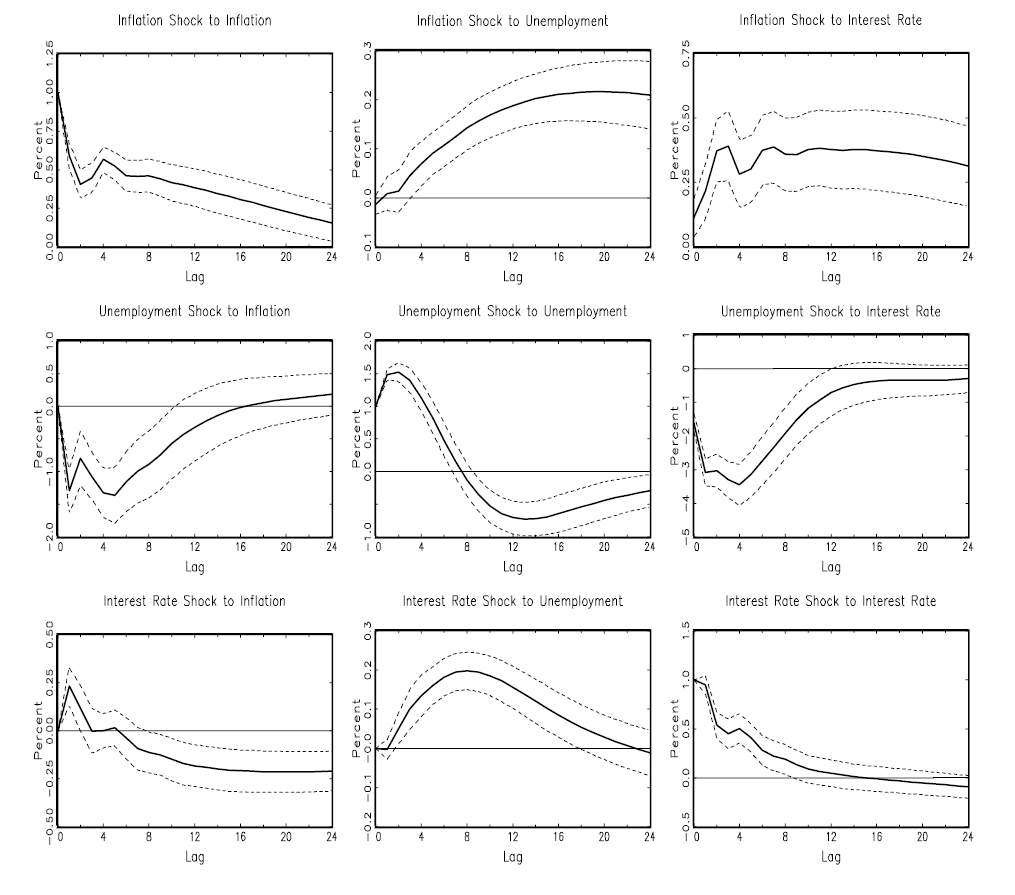
\includegraphics[width=0.75\linewidth]{IRF 1.png}
    \end{figure}
\end{frame}

\begin{frame}{Impulse Response Functions (IRF)}
\textbf{Objective: }analysing the effect of a given shock on a dynamic system, as proxied by a VAR variables.
\medskip
Assume the system receives a one-time shock of amplitude $\delta$ on the $j$-th structural innovation at time $t$:
        \[
        \varepsilon_{j,t} = \delta, 
        \qquad 
        \varepsilon_{j,t+1} = \varepsilon_{j,t+2} = \cdots = 0.
        \]

 The IRF traces out how each variable $y_{i,t+h}$ reacts at horizon $h$ to this one-time impulse.

\bigskip

\textbf{General definition:}
\[
I_{i,j,h}
= 
\frac{\partial\, y_{i,t+h}}{\partial\, \varepsilon_{j,t}}
\qquad (h = 0,1,2,\dots)
\]

\bigskip

For each horizon $h$, $I_h$ is a $k\times k$ matrix:
\[
I_h
=
\left[
\frac{\partial\, y_{i,t+h}}{\partial\, \varepsilon_{j,t}}
\right]_{i,j=1}^k
\]

\end{frame}


\begin{frame}{Impulse Response Functions (IRF)}
Dynamics of $y_t,\, y_{t+1},\, y_{t+2},\dots$ when $\varepsilon_t = 1,\ \varepsilon_{t+1}=0,\ \varepsilon_{t+2}=0,\dots$. \textbf{An IRF \textit{is the difference} between the forecast \textit{with the shock} and the forecast \textit{without the shock} (baseline).} It is \textbf{not} the raw forecast path itself after a shock.

\begin{figure}
    \centering
    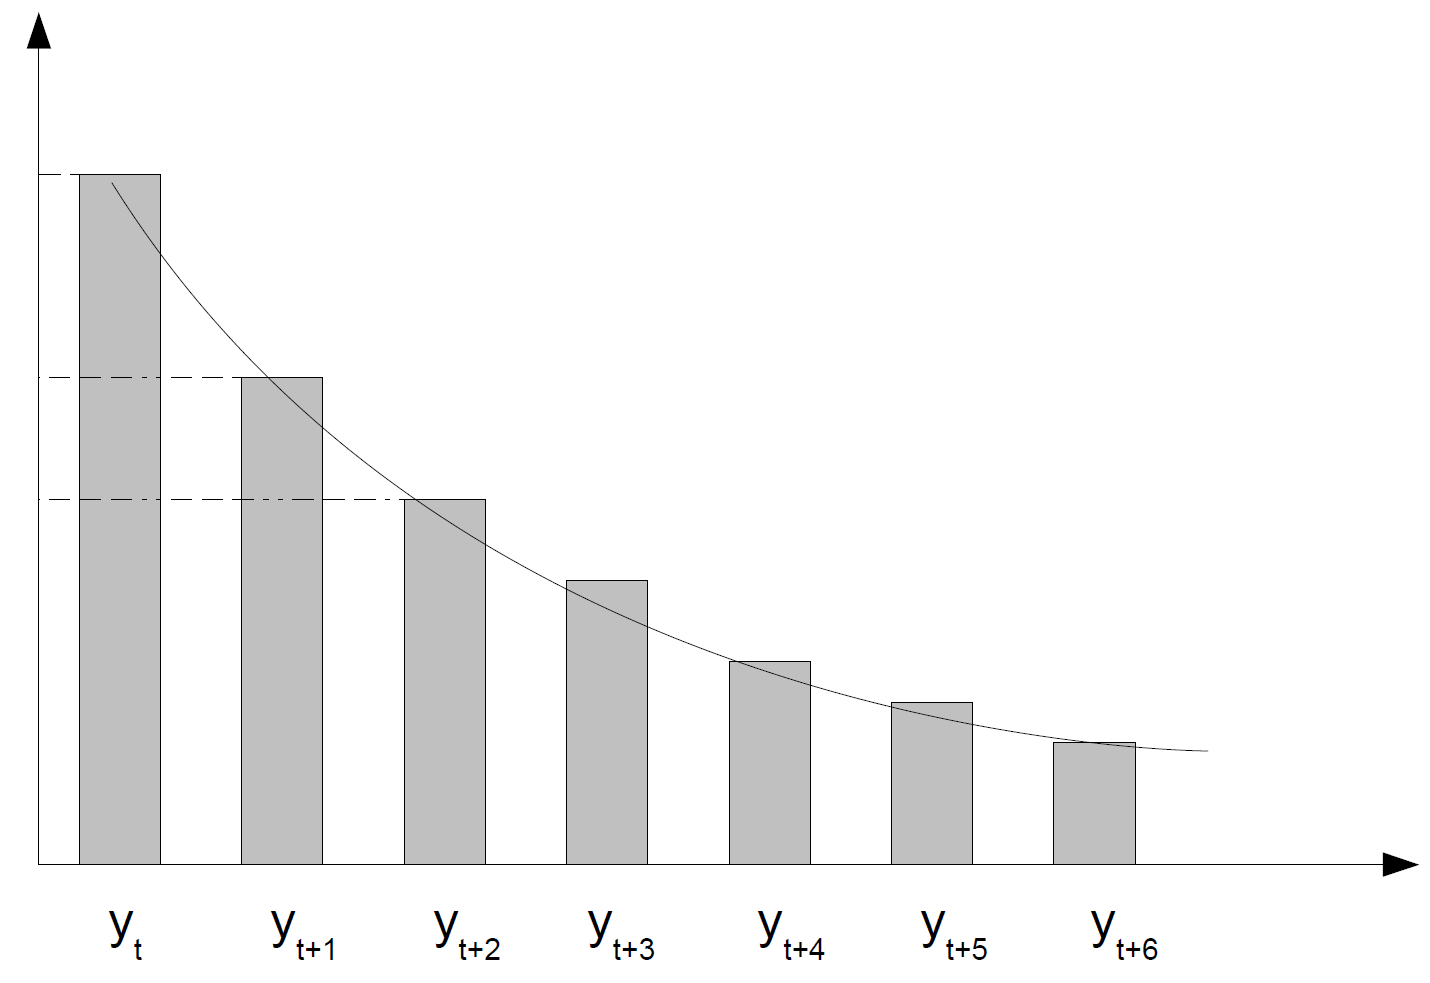
\includegraphics[width=0.75\linewidth]{irf 2.png}
\end{figure}
\end{frame}



%======================================================
\begin{frame}{IRFs from the VMA Representation}
%======================================================
\small

Consider the (zero-mean) structural VAR:
\[
\Phi(B) y_t = \varepsilon_t,
\qquad
\mathbb{E}[\varepsilon_t] = 0,
\qquad
\mathrm{Cov}(\varepsilon_t) = \Omega_\varepsilon.
\]

\medskip

If $\Phi(B)$ is invertible, we can express $y_t$ as a VMA($\infty$):
\[
y_t = \Phi(B)^{-1} \varepsilon_t
    = \Psi(B)\varepsilon_t
    = \varepsilon_t + \Psi_1 \varepsilon_{t-1}
                       + \Psi_2 \varepsilon_{t-2} + \cdots
\]

\bigskip

Then the impulse responses are simply:
\[
I_{i,j,h} = (\Psi_h)_{ij}
\]
Expectation based: 
\[
I_{i,j,h}
=
\mathbb{E}[y_{i,t+h} \mid \varepsilon_{j,t} = 1]
-
\mathbb{E}[y_{i,t+h} \mid \varepsilon_{j,t} = 0].
\]
\end{frame}



\begin{frame}{Impulse Response Functions (IRF)}
\small
\textbf{You must look at: }sign, magnitude, lag/delay, duration (short-term/long-term effects), mean-reversion or level change, overshooting (e.g. $+$ then $-$), significance (confidence intervals). 

\textbf{Reading:} impact of raw variable's shock on column variable. Diagonal = self-impact. 

\textbf{NB:} confidence intervals around IRFs are generally computed by Bootstrap
    \begin{figure}
        \centering
        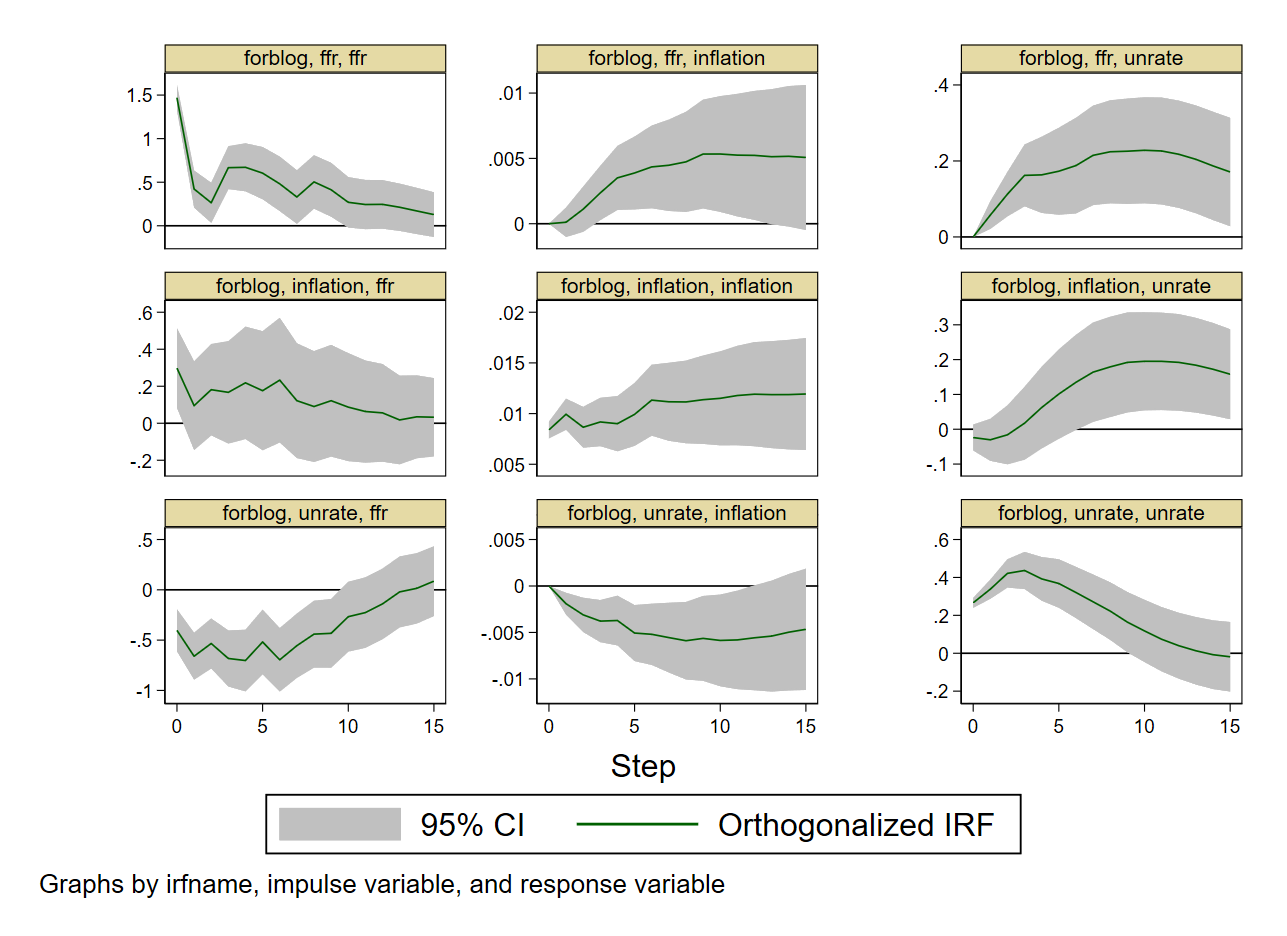
\includegraphics[width=0.75\linewidth]{irf 3.png}
    \end{figure}
\end{frame}

\begin{frame}{Impulse Response Functions (IRF) - Linearity}
\textbf{(SOME) LIMITS OF LINEARITY}
\smallskip
\begin{itemize}
    \item \textbf{As VARs are linear, a positive shock is the mirror image of a negative shock. }Only non-linear models can account for asymmetry.
    \begin{itemize}
        \item Always true in reality? \pause
        \item  Have the macro multipliers the same magnitude during expansion and during recession? E.g. Greek crisis (LMAO).
    \end{itemize}
    \item \textbf{As VARs are linear, the magnitude of the initial shock doesn’t matter in constructing the IRF.}
    \begin{itemize}
        \item Usually, a "unit shock" is a \textbf{one-standard-deviation shock} to the residual of a variable.
        \item 2.3 unit shock $\Longrightarrow$ 2.3 impulse response. 
        \item Always true in reality? \pause
        \item Thresholds? Tipping points? (e.g. the \textit{Great Moderation}, key rates and Minskyan moment). 
    \end{itemize}

\end{itemize}

\end{frame}


\begin{frame}{Forecast Error Variance Decomposition (FEVD)}
\footnotesize
\begin{itemize}
    \item The FEVD tells us \textbf{how much of the forecast error variance (i.e. uncertainty)} of a variable $y_{t}$ at horizon $h$ is explained by each structural shock in the VAR.

    \item When we forecast $y_{t+h}$, we make errors because future shocks ("innovations") are unknown. FEVD decomposes these forecast errors into \textbf{shares attributable to each shock}.
    
    \item The $h$-step forecast error is $y_{t+h} - \hat{y}_t(h)$  and its variance is given by the sum of the responses of future shocks:
    \[
       V\!\left(y_{t+h} - \hat{y}_t(h)\right)
       \;=\;
       \sum_{j=0}^{h-1} \Phi_j \, \Sigma_u \, \Phi_j'
    \]
    where $\Phi_j$ are the reduced-form moving-average matrices (same recursion as above), and $\Sigma_u$ is the covariance matrix of reduced-form innovations.

    \item The contribution of the \textbf{$i$-th orthogonalized shock} to the forecast error variance of the 
    \textbf{$k$-th variable} at horizon $h$ is:
    \[
       \sum_{j=0}^{h-1} 
       \left( e_k' \Psi_j e_i \right)^{\!2},
       \qquad \Psi_j = \Phi_j P
    \]
    where $P$ is the structural decomposition of $\Sigma_u = PP'$ (e.g.\ Cholesky) and $e_i$ selects the $i$-th orthogonalized shock.%
\end{itemize}

E.g. how much of GDP forecast uncertainty is explained by monetary policy shocks.

\end{frame}


\section{Causality?}

\begin{frame}{But what about \textit{\textbf{causality?}}}
So far: only \textit{\textbf{reduced-form}} VAR.
\medskip

Whereas the VAR model is able to capture efficiently the interactions between the different variables, it does not allow to reveal the underlying causal mechanisms since two different causal schemes can correspond to the same reduced forms.
\medskip

Innovation $u_{t,k}$ on variable $y_{t,k}$:\textbf{ no reason \textit{a priori} to be orthogonal} to the other variables (i.e. to be a "structural" shock")! Can be\textbf{ a contemporaneous feedback from the system!} Or can be the fruit of a \textbf{common shock on the whole system}!
\medskip

E.g. assessing the impact (IRF) of a monetary policy: an increase in interest rates in response to economic conditions is NOT considered as a shock, it is endogenous! Same for FEVD.
\medskip

\textbf{For next class!}
\end{frame}




\end{document}

